%; whizzy chapter
% -initex iniptex -latex platex -format platex -bibtex jbibtex -fmt fmt
% 以上 whizzytex を使用する場合の設定。

%     Tokyo Debian Meeting resources
%     Copyright (C) 2009 Junichi Uekawa
%     Copyright (C) 2009 Nobuhiro Iwamatsu
%     Copyright (C) 2009 Kohei Maeda

%     This program is free software; you can redistribute it and/or modify
%     it under the terms of the GNU General Public License as published by
%     the Free Software Foundation; either version 2 of the License, or
%     (at your option) any later version.

%     This program is distributed in the hope that it will be useful,
%     but WITHOUT ANY WARRANTY; without even the implied warranty of
%     MERCHANTABILITY or FITNESS FOR A PARTICULAR PURPOSE.  See the
%     GNU General Public License for more details.

%     You should have received a copy of the GNU General Public License
%     along with this program; if not, write to the Free Software
%     Foundation, Inc., 51 Franklin St, Fifth Floor, Boston, MA  02110-1301 USA

%  preview (shell-command (concat "evince " (replace-regexp-in-string "tex$" "pdf"(buffer-file-name)) "&"))
% 画像ファイルを処理するためにはebbを利用してboundingboxを作成。
%(shell-command "cd image200906; ebb *.png")

%%ここからヘッダ開始。

\documentclass[mingoth,a4paper]{jsarticle}
\usepackage{monthlyreport}
\usepackage{graphicx}

% 日付を定義する、毎月変わります。
% date --date 'third saturday'
\newcommand{\debmtgyear}{2009}
\newcommand{\debmtgmonth}{11}
\newcommand{\debmtgdate}{14}
\newcommand{\debmtgnumber}{58}

\begin{document}

\begin{titlepage}
\thispagestyle{empty}

% タイトルページ:編集必要な部分は最初のマクロに飛ばすこと

\vspace*{-2cm}
第\debmtgnumber{}回 東京エリア Debian 勉強会資料

\hspace*{-2.4cm}
\includegraphics[width=210mm]{image200801/2008title.eps}\\
\hfill{}\debmtgyear{}年\debmtgmonth{}月\debmtgdate{}日

\end{titlepage}


\newpage\mbox{}\newpage

\begin{minipage}[b]{0.2\hsize}
 \definecolor{titleback}{gray}{0.9}
 \colorbox{titleback}{\rotatebox{90}{\fontsize{80}{80} {\gt デビアン勉強会} }}
\end{minipage}
\begin{minipage}[b]{0.8\hsize}
\hrule
\vspace{2mm}
\hrule

% set depth to 1 if too many text, 2 if there's less
\setcounter{tocdepth}{1}
\tableofcontents
\vspace{2mm}
\hrule
\end{minipage}


\dancersection{Introduction}{上川 純一}

\begin{multicols}{2}
 
 
 今月のDebian勉強会へようこそ。これからDebianの世界にあしを踏み入れると
 いう方も、すでにどっぷりとつかっているという方も、月に一回Debianについ
 て語りませんか?

 Debian勉強会の目的は下記です。

 \begin{itemize}
 \item \underline{Debian Developer} (開発者)の育成。
 \item 日本語での「\underline{開発に関する情報}」を整理してまとめ、アップデートする。
 \item \underline{場}の提供。
 \begin{itemize}
  \item 普段ばらばらな場所にいる人々が face-to-face で出会える場を提供
	する。
  \item Debian のためになることを語る場を提供する。
  \item Debianについて語る場を提供する。
 \end{itemize}
 \end{itemize}		

 Debianの勉強会ということで究極的には参加者全員がDebian Packageをがりがり
 と作るスーパーハッカーになった姿を妄想しています。情報の共有・活用を通し
 て Debianの今後の能動的な展開への土台として、「場」としての空間を提供す
 るのが目的です。

 2009年の計画は仮です。

 \begin{enumerate}
  \item 新年の企画 (アンサンブル荻窪開催)
  \item OSC Tokyo
  \item VAIO P インストール記録、
	カーネル読書会 ディストリビューション大集合(小林さん)(東京大学?)
  \item Git Handson (岩松)(あんさんぶる荻窪?)
  \item 家Debianサーバ vs 職場のネットワーク(千代田区都立図書館?\footnote{\url{http://www.library.chiyoda.tokyo.jp/}})
  \item Asterisk (東京大学?)
  \item スペインにて開催
  \item Debconf報告会
  \item OSC Fall?
  \item udev + HAL(岩松さん)
  \item 3D graphics 開発(藤沢さん) 
  \item Debian サーバ+VMware + 各種OS、
	他の仮想化ツール(vserver etc.)、
	忘年会
 \end{enumerate}

 会場候補としては下記があります:

 \begin{itemize}
  \item 大学
  \item 恵比寿SGIホール
  \item Googleオフィス
  \item 公民館(あんさんぶる荻窪等)
  \item 都立会議室(無線LAN)
  \item 健保の施設
 \end{itemize}

\end{multicols}



\dancersection{事前課題}{上川 純一}

事前課題は:

「あなたが普段行っている統計処理の内容とその処理で行っているハックを披露
してください。」

この課題に対して提出いただいた内容は以下です。

\begin{multicols}{2}
%; whizzy-master ../debianmeetingresume200911.tex
% $B0J>e$N@_Dj$r$7$F$$$k$?$a!"$3$N%U%!%$%k$G(B M-x whizzytex $B$9$k$H!"(Bwhizzytex$B$,MxMQ$G$-$^$9!#(B

\begin{prework}{hoge}
\preworksection{hoge}


\end{prework}

\begin{prework}{fuga}

\preworksection{fuga}

\end{prework}

\begin{prework}{$B$^$($@$3$&$X$$(B}
\preworksection{$B$^$($@$3$&$X$$(B}

 $B8=>l$K$$$k$H$-$O$"$^$jI,MW$H$7$J$+$C$?$N$G$9$,!":rG/EY$^$G$N%W%j%;!<%k%9(B
 $B$N$H$-$O!"%W%m%S%8%g%K%s%0$9$k>e$G$N(BCPU$B$d%a%b%j$N%j%=!<%9;HMQN(!"8+@Q$j(B
 $B;n;;!"Gd>e;n;;!"8=>u$N4k2h$N;E;v$G$O!"?75,4k2h$H$N8=>u%5!<(B $B%S%9$NMxMQNL!"(B
 $BNA6b$NBPHf$J$I$r9T$&:]$KE}7W$r9T$C$?$j$7$F$$$^$9!#(B

 $B$,!"(BExcel$B$,CY$$$s$G$9$h$M!#(B5$BNs(B2$BK|9TDxEY$N7W;;$d!"%0%i%U$N%W%m%C%H$r9T$&(B
 $B$H!"$b$&Mn$A$kMn$A$k!#(BOS$B$N%l%9%]%s%9$bHs>o$K0-2=$7$F!":rG/$d$C$F$?0lHV(B
 $B9s$$Nc$G$O!"(B5$BJ,$K(B1$BEY!"(BExcel$B$,Mn$A$F!"%G!<%?I|5l$7$F$O%0%i%U:n$C$F$^$?Mn(B
 $B$A$F!"$J$s$F$H$-$K!"$b$&(BExcel$B$@$1$G$J$/%9%W%l%C%I%7!<%H$O7y$@$J$H;W$$$^(B
 $B$7$?!#(B

 $B7k2L$,J,$+$C$F$$$kE}7W%G!<%?$r%W%m%C%H$9$k$@$1$J$i%9%W%l%C%I%7!<%H$G$b(B
 $BNI$$$N$+$b$7$l$^$;$s$,!"CM$N%3%T!<$@$1$r$9$k$H!"$"$H$G8+D>$7$?$H$-$K!"(B
 $B$3$N%G!<%?$O$I$l$+$i;;=P$7$?$N$@$C$?$N$+$rGD0.$G$-$J$/$J$j$^$9!#$G$b%;(B
 $B%k$N;2>H$rB?MQ$9$k$HA0=R$NLdBj$OIQH/$7$d$9$/$J$j$^$9!#$9$k$H!"%G!<%?2r(B
 $B@O$7$?$j%0%i%UIA2h$O$b$&%9%W%l%C%I%7!<%H$O;_$a$?$$$J!"$H$$$&$N$,$-$C$+(B
 $B$1$G(B gnuplot $B$r;H$$;O$a$^$7$?!#$3$l$O$3$l$GJXMx$G$9$,:#2s$N%M%?H/I=$9$k(B
 $B$N$KEv$?$C$F!"(BGNU R$B$r;H$C$F$_$?$i!"$3$l$O$5$i$KJXMx$G$9$M!#;E;v$G$b$C$H(B
 $B3hMQ$7$h$&$H;W$$$^$9!#(B


 $B%W%i%$%Y!<%H$O!":#2s$N%M%?$N%5%s%W%k%G!<%?$N$h$&$J8wG.Hq$d!"2H7WJm$NE}7W(B
 $B$r<h$k$N$K(B OOo $B$r;H$C$F$^$7$?$,!"$3$l$b$d$C$Q$j%G!<%?$r=P$9$N$,LLE]$J$N(B
 $B$G!"$3$N5!2q$KJQ99$7$h$&$H;W$C$F$^$9!#(BOOo$B<+BN$b;_$a$h$&$+$J!#(B
\end{prework}

\begin{prework}{$BF|HfLn(B $B7<(B}
\preworksection{$BIaCJ9T$C$F$$$kE}7W=hM}$NFbMF$H$=$N=hM}$G9T$C$F$$$k%O%C%/(B}

 $BIaCJ!"E}7W=hM}$N$h$&$J$3$H$r$[$H$s$I$d$i$J$$$N$G$9$,!"(B2,3$BG/A0$K!"(B
 $B<+J,$N3+H/8zN($r7WB,$9$k$?$a$K!"(BOpenOffice.org $B$NI=7W;;5!G=$G(B
 $B%7%9%F%`3+H/$K$+$1$?;~4V$r:Y$+$/7WB,$7$F$_$?$3$H$,$"$j$^$9!#(B
 $B$d$`$r$($:<j:n6H$K$J$C$F$$$kK\Mh<+F02=$G$-$=$&$JItJ,$"$j!"(B
 libspreadsheet-writeexcel-perl $B$"$?$j$G2?$H$+$G$-$J$$$+5$$K$J$C$F$$$^$7$?!#(B
 $B$^$?5!2q$,$"$l$P;n$7$F$_$?$$$H;W$C$F$$$^$9!#(B
 R$B$N$h$&$J=hM}7O$b:#F|$r$-$C$+$1$K;H$$$3$J$;$k$h$&$K$7$F$*$-$?$$$H$3$m$G$9!#(B

\end{prework}


\end{multicols}

% image200911/prework.tex 内部にテキストを追加してください。
%
%

\dancersection{最近のDebian関連のミーティング報告}{前田耕平}
\subsection{東京エリアDebian勉強会56回目報告}
% (query-replace-regexp "<.*?>" "")
% (query-replace-regexp "^[	 ]\+" "")

56回は9月16日(水)19:00からといういつもとかなり変則的な時間で、ミラクルリ
ナックスさんのセミナールームをお借りして、Key Sign Party を行いました。
最初に岩松さんによる、なぜヒトはキーサインを求めるのか?というありがたい
お言葉をいただき、キーサインはWeb of Trustと言いつつも、その実はWeb of I
know whoでの信頼レベルなので、パスポートのような強力な公的な身分証明書で
己れの存在証明をする必要があるというはなしも途中ありました。100人もキー
サインする相手がいるとgpgコマンドでちまちまとやってられんよね?という問
題を解決する便利なツールcaffの使い方を伝授してもらいました。

その後、実際に参加したメンバー全員で、立食パーティでのキーサインパーティを
行いました。

参加された方は皆、リア充できたようです。

\subsection{東京エリアDebian勉強会57回目報告}
% (query-replace-regexp "<.*?>" "")
% (query-replace-regexp "^[	 ]\+" "")

第57回は、10月30日(金)、31日(土)に日本工学院大学の蒲田キャンパス12号館でOSC
2009Tokyo/Fallでブースのみ出展しました。元々は、31日のみ出展するでしたが、
あけどさんなど有志の方により、30日 (金) もブースをやっていたとのことです。

配布物としてはフライヤー50部、9月の勉強会で使用した GPG サインの資料20部、
Live DVD 20枚あまりを用意しました。また、展示物として岩松さんが sh7724
搭載マシンを用意してくれ、またそのマシンの詳細を印刷したパンフレットも用
意してくれました。
配布物の配布結果はほぼ予想通りで、そこそこ足りていました。
Live DVD のイメージが当日早朝にできたこともあり、ブースで少し焼きました
が、全部で25枚程度でした。

Live USB イメージ (lenny で lxde) も用意しましたが、案内が直前だったこと
もあるのか、あまり知られておらず、イメージを欲しがる人はそれほどいません
でした。ただし、30日 (金) にいらした方で、あけどさんに USB メモリを渡し
たまま帰ってしまった人がいたらしく、あけどさんが ML で連絡を求めています。
\footnote{\url{http://lists.debian.or.jp/debian-users/200911/msg00001.html} \\
\url{http://lists.debian.or.jp/debian-devel/200911/msg00000.html}}

また、岩松さん提案の GPG 鍵交換ですが、なかなか好評で、ブースおよび懇親
会で行ないました。

また、学生との交流もできたので、Debconf in Japanや出張Debian勉強会・
Debian温泉の企画にも進展がありそうです。

懇親会は JR 蒲田駅東口近くの「春香園」という餃子屋さんで行ないました。
懇親会の参加者は、武藤さん、上川さん夫妻、日比野さん、本庄さん、谷口さん、
岩松さん、藤澤さん、山本さん、前田の10名でした。

%============================================================
%%% trivia quiz
\dancersection{Debian Trivia Quiz}{上川 純一}

ところで、みなさん Debian 関連の話題においついていますか?Debian関連の話
題はメーリングリストをよんでいると追跡できます。ただよんでいるだけではは
りあいがないので、理解度のテストをします。特に一人だけでは意味がわからな
いところもあるかも知れません。みんなで一緒に読んでみましょう。

今回の出題範囲は\url{debian-devel-announce@lists.debian.org} に投稿された
内容とDebian Project Newsからです。

\begin{multicols}{2}
 %; whizzy-master ../debianmeetingresume200906.tex
% 以上の設定をしているため、このファイルで M-x whizzytex すると、whizzytexが利用できます。
%
% ちなみに、クイズは別ブランチで作成し、のちにマージします。逆にマージし
% ないようにしましょう。
% (shell-command "git checkout quiz-prepare")

\santaku
{新しくDebian keyring-mainterになったのは?}
{Kenshi Muto}
{Gunnar Wolf}
{Jonathan McDowell}
{B}
{}

\santaku
{次期リリース: Squeezeでサポート対象から落ちそうなアーキテクチャは?}
{alphaとhppa}
{i386とia64}
{s390とsparc}
{A}
{}

\santaku
{次期リリース: Squeezeで採用されるLinuxカーネルのバージョンは?}
{2.6.31}
{2.6.32}
{2.6.33}
{B}
{}

\santaku
{追加されたパッケージのオートリジェクトは何がトリガーになる?}
{妻帯者か否か}
{FTBFSのチェック}
{lintianによるパッケージチェック}
{C}
{}

\santaku
{Debconf10 はいつから開催されることになったか}
{2010年8月1日}
{2010年1月1日}
{2010年4月1日}
{A}
{}

\santaku
{Eugene V. Lyubimkinが発表したAPTの代替アプリケーションは?}
{debmoe}
{cupt}
{saitama}
{B}
{}

\end{multicols}

\clearpage

% ===============================================================
\dancersection{Debianでの数学ことはじめ。}{まえだこうへい}
\index{GNU R}
\index{GNU Octave}
\index{Gnuplot}
% ===============================================================

\subsection{はじめに}

Debianで数値計算や統計処理、グラフ作成を行うには、様々なパッケージがあり
ます。私のように大学での専行が理系といっても基礎生物学だった人間には、コン
ピュータでの専用ツールでなくても、極端な話、基本的な統計学と関数電卓があ
れば事足りました。スプレッドシートを使っても、関数は使わずに電卓代わりに
使うことも多かったと記憶してます\footnote{理由は、当時のスプレッドシート
の関数の精度が低く、自分で計算式を作った方が確実だったためです。今では改
善されたのでしょうか?}。社会人になってからもその延長でスプレッドシート
で大抵は事足りる、という方が一般的には多いのではないかと思います。

とはいえ、数万単位のサンプル数の計算をしたり、グラフを描写する場合、スプレッ
ドシートでは非力だという問題もあります。プリセールスや企画で裏付け資料を
作るのにサンプルデータを統計処理したり、データをプロットしてグラフを描く
と、スプレッドシートだとマウスの操作だけで簡単にできる一方、CPUやメモリ
不足でレスポンスが遅くなったり、ソフトウェア自体が落ちたり、酷いとOS自体
のレスポンスも悪化するというのが最近の仕事上での悩みだったりします。

そんなことがきっかけで今頃、Gnuplotを使い始めたわけですが、統計処理では
最近はRの書籍を書店で見かけたり、数値計算ではOctaveというのがあると
いうことをDebian勉強会のMLで知ったり\footnote{RやOctaveのパッケージ
メンテナであるDirk Eddelbuettel さんが近々来日されるというのがMLで流れて
いたそもそものきっかけです。\url{http://dirk.eddelbuettel.com/}}と、自分
の中だけでなく、最近意外とまわりでもこの辺はホットな話題ではないかと思い
ます。そこで、今回は私と同じように入門者向けに Octave、Gnuplotとの連携方
法、Rの話に加え、Debianでの使い方、パッケージングなどについて説明しよう
と思います。


\subsection{概要}
GNU Ocatave は計算処理のための高級言語で、MATLABという数値計算の商用ソフ
トウェアとの互換性があるようです。行列計算、連立方程式、微分・積分、グラ
フ出力などに使えます。グラフ描画のためには、gnuplotが必要です。

一方、GNU Rは統計解析のためのプログラミング言語で、文法的には、S言語や
Schemeに影響を受けているようです。Octaveとは異なり、グラフ描画には
gnuplotは必要ないようです。Excelなどのデータ読み込みができるといった、デー
タの互換性にも特徴があります。


\subsection{インストール方法}

Debian での各実行環境の導入方法について見てみます。今回の前提条件として、
ディストリビューションは Sid\footnote{2009年11月10日現在。}としています
が、Stable(Lenny)や Testing(Squeeze)でもバージョンが異なることを除けばほ
ぼ同じです。適宜読み替えてください。

\subsubsection{Octaveのインストール方法}

GNU OctaveはSqueeze/Sidでは、\texttt{octave}というパッケージ名ではなく、
バージョン3.0と3.2で別のパッケージになっています。今回は3.2のパッケージ
を導入します。

\begin{commandline}
$ sudo apt-get install octave3.2
\end{commandline}

\subsubsection{GNU Rのインストール方法}

GNU Rは、Debianパッケージでの名前は、gnurでも、rでもgnu-rでもありません。
\texttt{r-base}というメタパッケージで提供されています。これをインストールすると、
最低限、\texttt{r-base-core}パッケージがGNU Rの実行には必要です。また、GNU Rには、
機能拡張のパッケージが用意されています。CRAN(the Comprehensive R Archive
Network)からダウンロードできます。Perlでの CPAN のような位置づけです。
千以上ものパッケージがあるようです。Debianでは、CPANや Ruby gemsと同様に
ここから直接ダウンロードすることもできますが、約150のRパッケージがdebパッ
ケージとして用意されています\footnote{2009年11月9日現在。}。パッケージ名
は''\texttt{r-cran-<name>}''というネーミングルールです。

今回は\texttt{r-base}をインストールしましたが、余計なパッケージを入れな
いようにと、\texttt{r-base-core}パッケージをインストールしたとしても最小
構成からのパッケージの差は二つしかありません。\footnote{一つは\texttt{r-base}, も
う一つは\texttt{r-base-dev}です。}

\begin{commandline}
$ sudo apt-get install r-base
\end{commandline}

\subsubsection{Gnuplotのインストール}

GnuplotはOctave、GNU Rのいずれもdebパッケージとしての依存関係はありませ
んが、octaveではgnuplotを使ってグラフ描画もできるので、インストールして
おくと便利でしょう。gnuplotのインストールには\texttt{gnuplot}パッケージ
をインストールします。

\begin{commandline}
$ sudo apt-get install gnuplot
\end{commandline}

\subsection{試してみる。}

今回は、我が家の過去9年分の光熱費における各使用量の分布をサンプルデータ
としてみます。まずは、もともと使い始めていた gnuplot での例をみて、それ
に対し、Octave, R ではどのように処理するのかを見てみましょう。

用意したサンプルデータは以下のようなものです。

\begin{commandline}
"date","days","kWh","kWh/d","yen/d","yen","days","m^3","m^3/d","yen/d","yen","days","m^3","m^3/d","yen/d","yen","yen/d","yen"
2001/04,11,34,3.09,83.5,918,36,4.9,0.14,108.3,3900,58,9,0.16,22.8,1320,,
2001/05,33,95,2.88,73.8,2434,29,3.5,0.12,114.1,3310,,,,,,,
2001/06,30,129,4.3,102.7,3082,32,3,0.09,96.9,3100,61,3,0.05,15.7,960,,
2001/07,28,155,5.54,131.3,3676,28,1.7,0.06,91.1,2550,,,,,,,
(snip)
\end{commandline}

左から、年月,電気使用日数,月の電気使用量(kWh),1日あたりの電気使用量,1日
あたりの電気代,月の電気代,ガス使用日数,月のガス使用量(立方メートル),1日
あたりのガス使用量,1日あたりのガス代,月のガス代,水道使用日数,水道使用量
(立方メートル),1日あたりの水道使用量,1日あたりの水道代,月の水道代,1日あ
たりの下水道代,月の下水道代、となっています。

\subsubsection{gnuplot の場合}

gnuplotでは、次のようなバッチファイルを用意します。2001年4月から 2009年8
月までの電気、ガス、水道の各使用量をそれぞれプロットします。また、Debian
勉強会資料用に、LaTeXで取り込めるように、図はEPS、文字列はLaTeXで出力す
るようにします。

\begin{commandline}
reset
set terminal epslatex input color
set output "gnuplot.tex"
set datafile separator ","
set xdata time
set timefmt "%Y/%m"
set format x "%Y/%m"
set xtics rotate by -90
set mxtics 12
set xrange ["2001/04":"2009/08"]
set yrange [0:400]
set xlabel "年月"
set ylabel "電気使用量 [kWh]"
set y2range [0:50]
set y2label "ガス・水道使用量 [立方メートル]"
set ytics nomirror
set y2tics
plot "kohnetsuhi.csv" using 1:3 axes x1y1 title "電気" with line,\
     "" using 1:8 axes x1y2 title "ガス" with line,\
     "" using 1:13 axes x1y2 title "水道" with line
\end{commandline}

このバッチファイルをLaTeXとEPSに変換します。バッチファイルをロードするに
は、対話モードでloadコマンドを実行します。

\begin{commandline}
$ gnuplot

	G N U P L O T
	Version 4.2 patchlevel 6 
	last modified Sep 2009
	System: Linux 2.6.31.3

	Copyright (C) 1986 - 1993, 1998, 2004, 2007 - 2009
	Thomas Williams, Colin Kelley and many others

	Type `help` to access the on-line reference manual.
	The gnuplot FAQ is available from http://www.gnuplot.info/faq/

	Send bug reports and suggestions to <http://sourceforge.net/projects/gnuplot>


Terminal type set to 'wxt'
gnuplot> load ``gnuplot.gp''
gnuplot> quit
\end{commandline}

これで、カレントディレクトリに gnuplot.texとgnuplot.epsファイルが出力さ
れます。gnuplot.tex は、LaTeX文書の中で以下のように記述して取り込みます。

\begin{commandline}
\usepackage{graphicx}

(snip)

\begin{figure}[thbp]
% GNUPLOT: LaTeX picture with Postscript
\begingroup
  \makeatletter
  \providecommand\color[2][]{%
    \GenericError{(gnuplot) \space\space\space\@spaces}{%
      Package color not loaded in conjunction with
      terminal option `colourtext'%
    }{See the gnuplot documentation for explanation.%
    }{Either use 'blacktext' in gnuplot or load the package
      color.sty in LaTeX.}%
    \renewcommand\color[2][]{}%
  }%
  \providecommand\includegraphics[2][]{%
    \GenericError{(gnuplot) \space\space\space\@spaces}{%
      Package graphicx or graphics not loaded%
    }{See the gnuplot documentation for explanation.%
    }{The gnuplot epslatex terminal needs graphicx.sty or graphics.sty.}%
    \renewcommand\includegraphics[2][]{}%
  }%
  \providecommand\rotatebox[2]{#2}%
  \@ifundefined{ifGPcolor}{%
    \newif\ifGPcolor
    \GPcolortrue
  }{}%
  \@ifundefined{ifGPblacktext}{%
    \newif\ifGPblacktext
    \GPblacktexttrue
  }{}%
  % define a \g@addto@macro without @ in the name:
  \let\gplgaddtomacro\g@addto@macro
  % define empty templates for all commands taking text:
  \gdef\gplbacktext{}%
  \gdef\gplfronttext{}%
  \makeatother
  \ifGPblacktext
    % no textcolor at all
    \def\colorrgb#1{}%
    \def\colorgray#1{}%
  \else
    % gray or color?
    \ifGPcolor
      \def\colorrgb#1{\color[rgb]{#1}}%
      \def\colorgray#1{\color[gray]{#1}}%
      \expandafter\def\csname LTw\endcsname{\color{white}}%
      \expandafter\def\csname LTb\endcsname{\color{black}}%
      \expandafter\def\csname LTa\endcsname{\color{black}}%
      \expandafter\def\csname LT0\endcsname{\color[rgb]{1,0,0}}%
      \expandafter\def\csname LT1\endcsname{\color[rgb]{0,1,0}}%
      \expandafter\def\csname LT2\endcsname{\color[rgb]{0,0,1}}%
      \expandafter\def\csname LT3\endcsname{\color[rgb]{1,0,1}}%
      \expandafter\def\csname LT4\endcsname{\color[rgb]{0,1,1}}%
      \expandafter\def\csname LT5\endcsname{\color[rgb]{1,1,0}}%
      \expandafter\def\csname LT6\endcsname{\color[rgb]{0,0,0}}%
      \expandafter\def\csname LT7\endcsname{\color[rgb]{1,0.3,0}}%
      \expandafter\def\csname LT8\endcsname{\color[rgb]{0.5,0.5,0.5}}%
    \else
      % gray
      \def\colorrgb#1{\color{black}}%
      \def\colorgray#1{\color[gray]{#1}}%
      \expandafter\def\csname LTw\endcsname{\color{white}}%
      \expandafter\def\csname LTb\endcsname{\color{black}}%
      \expandafter\def\csname LTa\endcsname{\color{black}}%
      \expandafter\def\csname LT0\endcsname{\color{black}}%
      \expandafter\def\csname LT1\endcsname{\color{black}}%
      \expandafter\def\csname LT2\endcsname{\color{black}}%
      \expandafter\def\csname LT3\endcsname{\color{black}}%
      \expandafter\def\csname LT4\endcsname{\color{black}}%
      \expandafter\def\csname LT5\endcsname{\color{black}}%
      \expandafter\def\csname LT6\endcsname{\color{black}}%
      \expandafter\def\csname LT7\endcsname{\color{black}}%
      \expandafter\def\csname LT8\endcsname{\color{black}}%
    \fi
  \fi
  \setlength{\unitlength}{0.0500bp}%
  \begin{picture}(7200.00,5040.00)%
    \gplgaddtomacro\gplbacktext{%
      \csname LTb\endcsname%
      \put(1210,1408){\makebox(0,0)[r]{\strut{} 0}}%
      \put(1210,1829){\makebox(0,0)[r]{\strut{} 50}}%
      \put(1210,2250){\makebox(0,0)[r]{\strut{} 100}}%
      \put(1210,2671){\makebox(0,0)[r]{\strut{} 150}}%
      \put(1210,3092){\makebox(0,0)[r]{\strut{} 200}}%
      \put(1210,3513){\makebox(0,0)[r]{\strut{} 250}}%
      \put(1210,3934){\makebox(0,0)[r]{\strut{} 300}}%
      \put(1210,4355){\makebox(0,0)[r]{\strut{} 350}}%
      \put(1210,4776){\makebox(0,0)[r]{\strut{} 400}}%
      \put(1763,1276){\rotatebox{-90}{\makebox(0,0)[l]{\strut{}2002/01}}}%
      \put(2320,1276){\rotatebox{-90}{\makebox(0,0)[l]{\strut{}2003/01}}}%
      \put(2877,1276){\rotatebox{-90}{\makebox(0,0)[l]{\strut{}2004/01}}}%
      \put(3436,1276){\rotatebox{-90}{\makebox(0,0)[l]{\strut{}2005/01}}}%
      \put(3994,1276){\rotatebox{-90}{\makebox(0,0)[l]{\strut{}2006/01}}}%
      \put(4551,1276){\rotatebox{-90}{\makebox(0,0)[l]{\strut{}2007/01}}}%
      \put(5107,1276){\rotatebox{-90}{\makebox(0,0)[l]{\strut{}2008/01}}}%
      \put(5667,1276){\rotatebox{-90}{\makebox(0,0)[l]{\strut{}2009/01}}}%
      \put(6122,1408){\makebox(0,0)[l]{\strut{} 0}}%
      \put(6122,2082){\makebox(0,0)[l]{\strut{} 10}}%
      \put(6122,2755){\makebox(0,0)[l]{\strut{} 20}}%
      \put(6122,3429){\makebox(0,0)[l]{\strut{} 30}}%
      \put(6122,4102){\makebox(0,0)[l]{\strut{} 40}}%
      \put(6122,4776){\makebox(0,0)[l]{\strut{} 50}}%
      \put(440,3092){\rotatebox{90}{\makebox(0,0){\strut{}$BEE5$;HMQNL(B [kWh]}}}%
      \put(6759,3092){\rotatebox{90}{\makebox(0,0){\strut{}$B%,%9!&?eF;;HMQNL(B [$BN)J}%a!<%H%k(B]}}}%
      \put(3666,154){\makebox(0,0){\strut{}$BG/7n(B}}%
    }%
    \gplgaddtomacro\gplfronttext{%
      \csname LTb\endcsname%
      \put(5003,4603){\makebox(0,0)[r]{\strut{}$BEE5$(B}}%
      \csname LTb\endcsname%
      \put(5003,4383){\makebox(0,0)[r]{\strut{}$B%,%9(B}}%
      \csname LTb\endcsname%
      \put(5003,4163){\makebox(0,0)[r]{\strut{}$B?eF;(B}}%
    }%
    \gplbacktext
    \put(0,0){\includegraphics{image200911/gnuplot.eps}}%
    \gplfronttext
  \end{picture}%
\endgroup

\end{figure}
\end{commandline}

ただし、このままでは make が通りません。gnuplot.tex を書き換える必要があ
ります。次のように下から3行目の includegraphicsのパスを変更する必要があ
ります。

\begin{commandline}

$ diff -u gnuplot.tex.bk gnuplot.tex
--- gnuplot.tex.orig	2009-11-12 23:38:36.000000000 +0900
+++ gnuplot.tex	2009-11-12 23:39:39.000000000 +0900
@@ -111,7 +111,7 @@
       \put(5003,4163){\makebox(0,0)[r]{\strut{}水道}}%
     }%
     \gplbacktext
-    \put(0,0){\includegraphics{gnuplot}}%
+    \put(0,0){\includegraphics{image200911/gnuplot.eps}}%
     \gplfronttext
   \end{picture}%
 \endgroup
\end{document}
\end{commandline}

これで make すると、以下のような図を表示できます。

\begin{figure}[thbp]
 % GNUPLOT: LaTeX picture with Postscript
\begingroup
  \makeatletter
  \providecommand\color[2][]{%
    \GenericError{(gnuplot) \space\space\space\@spaces}{%
      Package color not loaded in conjunction with
      terminal option `colourtext'%
    }{See the gnuplot documentation for explanation.%
    }{Either use 'blacktext' in gnuplot or load the package
      color.sty in LaTeX.}%
    \renewcommand\color[2][]{}%
  }%
  \providecommand\includegraphics[2][]{%
    \GenericError{(gnuplot) \space\space\space\@spaces}{%
      Package graphicx or graphics not loaded%
    }{See the gnuplot documentation for explanation.%
    }{The gnuplot epslatex terminal needs graphicx.sty or graphics.sty.}%
    \renewcommand\includegraphics[2][]{}%
  }%
  \providecommand\rotatebox[2]{#2}%
  \@ifundefined{ifGPcolor}{%
    \newif\ifGPcolor
    \GPcolortrue
  }{}%
  \@ifundefined{ifGPblacktext}{%
    \newif\ifGPblacktext
    \GPblacktexttrue
  }{}%
  % define a \g@addto@macro without @ in the name:
  \let\gplgaddtomacro\g@addto@macro
  % define empty templates for all commands taking text:
  \gdef\gplbacktext{}%
  \gdef\gplfronttext{}%
  \makeatother
  \ifGPblacktext
    % no textcolor at all
    \def\colorrgb#1{}%
    \def\colorgray#1{}%
  \else
    % gray or color?
    \ifGPcolor
      \def\colorrgb#1{\color[rgb]{#1}}%
      \def\colorgray#1{\color[gray]{#1}}%
      \expandafter\def\csname LTw\endcsname{\color{white}}%
      \expandafter\def\csname LTb\endcsname{\color{black}}%
      \expandafter\def\csname LTa\endcsname{\color{black}}%
      \expandafter\def\csname LT0\endcsname{\color[rgb]{1,0,0}}%
      \expandafter\def\csname LT1\endcsname{\color[rgb]{0,1,0}}%
      \expandafter\def\csname LT2\endcsname{\color[rgb]{0,0,1}}%
      \expandafter\def\csname LT3\endcsname{\color[rgb]{1,0,1}}%
      \expandafter\def\csname LT4\endcsname{\color[rgb]{0,1,1}}%
      \expandafter\def\csname LT5\endcsname{\color[rgb]{1,1,0}}%
      \expandafter\def\csname LT6\endcsname{\color[rgb]{0,0,0}}%
      \expandafter\def\csname LT7\endcsname{\color[rgb]{1,0.3,0}}%
      \expandafter\def\csname LT8\endcsname{\color[rgb]{0.5,0.5,0.5}}%
    \else
      % gray
      \def\colorrgb#1{\color{black}}%
      \def\colorgray#1{\color[gray]{#1}}%
      \expandafter\def\csname LTw\endcsname{\color{white}}%
      \expandafter\def\csname LTb\endcsname{\color{black}}%
      \expandafter\def\csname LTa\endcsname{\color{black}}%
      \expandafter\def\csname LT0\endcsname{\color{black}}%
      \expandafter\def\csname LT1\endcsname{\color{black}}%
      \expandafter\def\csname LT2\endcsname{\color{black}}%
      \expandafter\def\csname LT3\endcsname{\color{black}}%
      \expandafter\def\csname LT4\endcsname{\color{black}}%
      \expandafter\def\csname LT5\endcsname{\color{black}}%
      \expandafter\def\csname LT6\endcsname{\color{black}}%
      \expandafter\def\csname LT7\endcsname{\color{black}}%
      \expandafter\def\csname LT8\endcsname{\color{black}}%
    \fi
  \fi
  \setlength{\unitlength}{0.0500bp}%
  \begin{picture}(7200.00,5040.00)%
    \gplgaddtomacro\gplbacktext{%
      \csname LTb\endcsname%
      \put(1210,1408){\makebox(0,0)[r]{\strut{} 0}}%
      \put(1210,1829){\makebox(0,0)[r]{\strut{} 50}}%
      \put(1210,2250){\makebox(0,0)[r]{\strut{} 100}}%
      \put(1210,2671){\makebox(0,0)[r]{\strut{} 150}}%
      \put(1210,3092){\makebox(0,0)[r]{\strut{} 200}}%
      \put(1210,3513){\makebox(0,0)[r]{\strut{} 250}}%
      \put(1210,3934){\makebox(0,0)[r]{\strut{} 300}}%
      \put(1210,4355){\makebox(0,0)[r]{\strut{} 350}}%
      \put(1210,4776){\makebox(0,0)[r]{\strut{} 400}}%
      \put(1763,1276){\rotatebox{-90}{\makebox(0,0)[l]{\strut{}2002/01}}}%
      \put(2320,1276){\rotatebox{-90}{\makebox(0,0)[l]{\strut{}2003/01}}}%
      \put(2877,1276){\rotatebox{-90}{\makebox(0,0)[l]{\strut{}2004/01}}}%
      \put(3436,1276){\rotatebox{-90}{\makebox(0,0)[l]{\strut{}2005/01}}}%
      \put(3994,1276){\rotatebox{-90}{\makebox(0,0)[l]{\strut{}2006/01}}}%
      \put(4551,1276){\rotatebox{-90}{\makebox(0,0)[l]{\strut{}2007/01}}}%
      \put(5107,1276){\rotatebox{-90}{\makebox(0,0)[l]{\strut{}2008/01}}}%
      \put(5667,1276){\rotatebox{-90}{\makebox(0,0)[l]{\strut{}2009/01}}}%
      \put(6122,1408){\makebox(0,0)[l]{\strut{} 0}}%
      \put(6122,2082){\makebox(0,0)[l]{\strut{} 10}}%
      \put(6122,2755){\makebox(0,0)[l]{\strut{} 20}}%
      \put(6122,3429){\makebox(0,0)[l]{\strut{} 30}}%
      \put(6122,4102){\makebox(0,0)[l]{\strut{} 40}}%
      \put(6122,4776){\makebox(0,0)[l]{\strut{} 50}}%
      \put(440,3092){\rotatebox{90}{\makebox(0,0){\strut{}$BEE5$;HMQNL(B [kWh]}}}%
      \put(6759,3092){\rotatebox{90}{\makebox(0,0){\strut{}$B%,%9!&?eF;;HMQNL(B [$BN)J}%a!<%H%k(B]}}}%
      \put(3666,154){\makebox(0,0){\strut{}$BG/7n(B}}%
    }%
    \gplgaddtomacro\gplfronttext{%
      \csname LTb\endcsname%
      \put(5003,4603){\makebox(0,0)[r]{\strut{}$BEE5$(B}}%
      \csname LTb\endcsname%
      \put(5003,4383){\makebox(0,0)[r]{\strut{}$B%,%9(B}}%
      \csname LTb\endcsname%
      \put(5003,4163){\makebox(0,0)[r]{\strut{}$B?eF;(B}}%
    }%
    \gplbacktext
    \put(0,0){\includegraphics{image200911/gnuplot.eps}}%
    \gplfronttext
  \end{picture}%
\endgroup

 \caption{gnuplotでのプロットの例}
\end{figure}

では、これを Rではどのようにするのかを見てみましょう。\footnote{Octaveは
gnuplotを使ってグラフ描画するということなので、今回省略。手が回らなかっ
たのが事実ですが、何か。}

\subsubsection{GNU Rの場合}

GNU Rを対話形式で使うには、シェルで\texttt{R}と実行します。
\begin{commandline}
$ R
\end{commandline}

Rでデータを扱うには、先ほどの konetsu.csvファイルをオブジェクトに取り込
む必要があります。取り込むには、\verb/<-/演算子を使います。

\begin{commandline}
> konetsu <- read.csv("konetsu.csv")
\end{commandline}

この konetsu オブジェクトの中身を見てみます。このオブジェクトはデータフ
レームといい、これを指定するだけです。

\begin{commandline}
> konetsu
    X...date days kWh kWh.day yen.day  yen days.1  m.3 m.3.day yen.day.1 yen.1
1     2001/4   11  34    3.09    83.5  918     36  4.9    0.14     108.3  3900
2     2001/5   33  95    2.88    73.8 2434     29  3.5    0.12     114.1  3310
3     2001/6   30 129    4.30   102.7 3082     32  3.0    0.09      96.9  3100
4     2001/7   28 155    5.54   131.3 3676     28  1.7    0.06      91.1  2550
5     2001/8   34 212    6.24   146.9 4995     35  2.2    0.06      78.9  2760
(snip)
    days.2 m.3.1 m.3.day.1 fee.d yen.2 yen.day.2 yen.3
1       58     9      0.16  22.8  1320        NA    NA
2       NA    NA        NA    NA    NA        NA    NA
3       61     3      0.05  15.7   960        NA    NA
4       NA    NA        NA    NA    NA        NA    NA
5       60     6      0.10  19.0  1140        NA    NA
(snip)
\end{commandline}
 
列数が増えると、この例のように分割して表示されます。``NA''と表示されてい
るのは、値がnullだったものです。

また、この取り込んだデータのサマリを表示させることも簡単です。以下のよう
に Rでは統計処理のための関数があらかじめ用意されているので、とても便利で
す。

\begin{commandline}
> summary(konetsu)
    X...date       days            kWh           kWh.day          yen.day
 2006/9 : 2   Min.   :11.00   Min.   : 34.0   Min.   : 2.880   Min.   : 73.8
 2001/10: 1   1st Qu.:29.00   1st Qu.:170.2   1st Qu.: 5.753   1st Qu.:129.1
 2001/11: 1   Median :30.00   Median :195.0   Median : 6.410   Median :147.3
 2001/12: 1   Mean   :30.09   Mean   :199.1   Mean   : 6.565   Mean   :151.3
 2001/4 : 1   3rd Qu.:33.00   3rd Qu.:219.0   3rd Qu.: 7.225   3rd Qu.:171.0
 2001/5 : 1   Max.   :35.00   Max.   :363.0   Max.   :11.000   Max.   :250.1
 (Other):95
(snip)
\end{commandline}

各項目のデータを表示するには、データフレームのオブジェクト名と自動的につ
けられた変量名を \verb/データフレーム名$変量名/ で指定します。

\begin{commandline}
> konetsu$date
  [1] 2001/04 2001/05 2001/06 2001/07 2001/08 2001/09 2001/10 2001/11 2001/12
 [10] 2002/01 2002/02 2002/03 2002/04 2002/05 2002/06 2002/07 2002/08 2002/09
(snip)
[100] 2009/07 2009/08 2009/09
102 Levels: 2001/04 2001/05 2001/06 2001/07 2001/08 2001/09 2001/10 ... 2009/09
\end{commandline}

それでは、gnuplot の時と同じようにプロットしてみます。今回も EPSで出
力します。

\begin{commandline}
> postscript("gnur.eps", horizontal=FALSE, height=5, width=5, pointsize=10)
> plot(konetsu$kWh, type="l", ylim=c(0,400), ann=F)
> par(new=T)
> plot(konetsu$m.3, type="l", ylim=c(0,400), ann=F, col="red")
> par(new=T)
> plot(konetsu$m.3.1, ylim=c(0,400), ann=F, col="blue")
> dev.off()
X11cairo 
       2 
>
\end{commandline}

出力された、EPSをLaTeXに取り込むと以下の図のようになります。
\begin{figure}[H]
 \includegraphics[width=0.5\hsize]{image200911/gnur.eps}
 \caption{GNU Rでのプロットの例}
\end{figure}

第2軸だけに表示させる方法が分からなかったので、Y軸のスケールを全部同じに
しなくてはならなかったりと、gnuplot に比べると若干見づらくなってしまいま
した。もうちょっと修行が必要そうです。

\subsection{Debian の環境における注意点。}

ところで、Debian ではGNU RはCRANのパッケージがdebパッケージ化されていると上述しま
したが、GNU Octaveも Octave-Forge プロジェクトという、CRAN に相当する拡
張パッケージが、SorceForgeで公開されています
\footnote{\url{http://octave.sourceforge.net/packages.html}}。CRAN由来の
パッケージと違い、パッケージのネーミングルールは決まっていません。ただし、
現状では、Octaveそのものに由来するパッケージは、\verb/octaveX.X[-*]/という形で、
バージョンX.Xのブランチごとのパッケージ、名前になっています。一方、
Octave-Forgeをはじめ、拡張機能のパッケージは、\verb/octave-*/というパッ
ケージ名になっていますので、ある程度判断するための目安にはなるでしょう。

\begin{commandline}
$ apt-cache search "GNU R" | wc -l
213
$ apt-cache search octave | wc -l
133
\end{commandline}

それぞれ、debパッケージにする場合の考慮点を見てみましょう。

\subsubsection{Octaveの場合}

DebianにはOctave関連パッケージのメンテナンスチーム Debian Octave Group
が存在します\footnote{\url{http://pkg-octave.alioth.debian.org}}。debパッ
ケージに未だなっておらず、debパッケージにしたいソフトウェア、例えば、膨
大なCRAN パッケージを debパッケージ化したい場合、あるいは野良パッケージ
を作った場合などは、ITPする際に、Debian Octave
Group\footnote{pkg-octave-devel@lists.alioth.debian.org}にもCCを入れてお
くと良いでしょう。

また、README.Debianにも記載されていますが、OctaveのドキュメントにはPDFが含まれ
ているため、\texttt{octave3.0-doc, octave3.2-doc}という名前で拡張パッケー
ジとして提供されています。

Octaveパッケージのビルドには、\texttt{octave-pkg-dev}パッケージという専
用の環境が用意されています。Octave はバージョン3.0からアドオンを作成する
場合には、pkg.m systemという環境を使ってインストールするようになっていま
すが、これをDebian用のパッケージング環境として用意されています。

このパッケージを使ってパッケージを作るには、debian/controlの
Build-Dependsに、octave-pkg-devを、Dependsに\verb/${octave:Depends}/を追
記します。

また、debian/rules に

\begin{commandline}
 include /usr/share/cdbs/1/class/octave-pkg.mk
\end{commandline}

を追記する必要があります\footnote{octave-pkg-devパッケージのREADMEには、
include /usr/share/octave/debian/octave-pkg-dev.mkを追記するように記述さ
れていますが、バージョン0.5でファイル名の変更をしており、ドキュメントの
更新が追いついていないようです。}。

また、debian/rulesで、get-orig-sourceターゲットも透過的に提供されていま
す。これは前述のOctave-Forge プロジェクトからのパッケージの配布のみに作
用しています。アップストリームのパッケージがこのSourceForge以外からする
場合は、自分で get-orig-source ターゲットを定義できます。octave-pkg-dev
パッケージ特有のルールの実行を防ぐには、\texttt{''SOURCEFORGE = NO''}を
debian/rulesに設定する必要があります。

\subsubsection{GNU Rの場合}

GNU Rパッケージのビルドには、Octaveと同様、\texttt{r-base-dev}パッケージ
という専用のビルド環境が用意されています。ビルド時の対応として、Debian
パッケージポリシーの考慮が必要です。Rの実行ファイルは、
/usr/lib/R/bin/R.binary として分離されています。

私の環境では、上記のパスには以下のファイルが存在しますが、ここでは、
/usr/lib/R/bin/Rscriptが該当します。

\begin{commandline}
$ file /usr/lib/R/bin/R*
/usr/lib/R/bin/R:       Bourne-Again shell script text executable
/usr/lib/R/bin/REMOVE:  ASCII text
/usr/lib/R/bin/Rcmd:    Bourne-Again shell script text executable
/usr/lib/R/bin/Rd2dvi:  ASCII English text
/usr/lib/R/bin/Rdconv:  ASCII text
/usr/lib/R/bin/Rdiff:   Bourne-Again shell script text executable
/usr/lib/R/bin/Rprof:   a /usr/bin/perl script text executable
/usr/lib/R/bin/Rscript: ELF 64-bit LSB executable, x86-64, version 1 (SYSV), dynamically linked (uses shared libs), for GNU/Linux 2.6.18, stripped
\end{commandline}

\subsection{まとめ。}

今回は、Debian で数学ことはじめ、ということで、Octave, GNU R, gnuplotを
取り上げ、基本的な使い方と、ちょっと視点を変えて、拡張パッケージの
Debian パッケージのお作法についてお話しました。使い込んでいけばかなり便
利そうな印象があります。

数学、と言う観点からはかなりずれてしまいましたが、スプレッドシート地獄か
ら脱出しましょう。

\begin{thebibliography}{0}
 \bibitem{gnuplot-lecture}
   山本昌志
   「gnuplot の精義 フリーの高機能グラフ作成ツールを使いこなす」
\end{thebibliography}

\clearpage


\dancersection{Debian autobuilder ネットワーク}{岩松}

Debianは現時点で11個のCPUアーキテクチャと2つのカーネルをサポートしていま
す(i386, amd64, ppc, mips, mipsel, armel, alpha, ia64, s390, hppa,
sparc, kfreebsd-amd64, kfreebsd-i386)。

パッケージが数万個あり、パッケージメンテナが Debianのサーバにアップロー
ドすると、いつのまにかユーザが知らないうちに各アーキテクチャ向けにDebianパッケージがビルドされ、
利用できるようになっています。これはどのような仕組みで動いているのでしょ
うか。
もちろん、パッケージメンテナはすべてのアーキテクチャを持っているわけでは
ないので(持っている人もいるみたいですが。)、パッケージメンテナが各アー
キテクチャ毎にビルドして、アップロードしてわけではありません。
Debianでは {\bf Autobuilder ネットワーク} と呼ばれる 各アーキテクチャ向
けにパッケージが自動的にビルドされるシステムが行っています。
Debian Project では重要なシステムの一つなのですが、表に出てくる事も少な
いためどのような動きになっているのか知る人は少ないです。
今回、Renesas SuperH(SH4)を移植するにあたりこれらの情報を入手したの
でまとめてみました。また、新しくアーキテクチャを追加する時の方法と、ビル
ドテクニックについても説明します。

\subsection{Autobuilder ネットワークのコンポーネント}

Autobuilder ネットワーク は一つのソフトウェアで動いているわけではなく、
いくつかのソフトウェアと porter
と呼ばれる buildd のメンテナ、wanna-buildのメンテナで構成されています。
Autobuilder ネットワークの動きを説明する前に、各コンポーネントがど
のような動きをするのか説明します。

\subsubsection{dak}
Debian Archive Kit。
パッケージメンテナ/Builddによってアップロードされたパッケージをチェック、
管理するためのツールやデーモンが提供されています。

\subsubsection{quinn-diff}
パッケージメンテナによって新しくアップロードされたソフトウェアのアーキ
テクチャ依存のパッケージ (Archi-
tecture: any) とアーキテクチャ非依存のパッケージ (Architecture: all) を
チェックし、前者を wanna-build のデー
タベースに登録するツールです。これはソースパッケージだけでなく、バイナ
リパッケージもチェックします。
Autobuilder ネットワークの過程では アーキテクチャ非依存のパッケージはビ
ルドされません。

パッケージ情報: \url{http://packages.qa.debian.org/q/quinn-diff.html}

\subsubsection{wanna-build}
buildd とデータのやりとりをするためのインターフェイスです。各アーキテク
チャ毎にパッケージのデータベースを持ちます。
buildd は wanna-build のデータベースを持つサーバに ssh でログインし、
wanna-build コマンドを使ってデータベースをコントロールします。

パッケージ情報: \url{http://packages.debian.org/sid/wanna-build}

\subsubsection{buildd}
wanna-build と データをやりとりするデーモンやパッケージをアップロードす
るツール一式を指します。ツールには以下のものがあります。

パッケージ情報: \url{http://packages.debian.org/sid/buildd}

\begin{itemize}
\item buildd\\
  buildd デーモン。wanna-buildd のデータベースを定期的にチェックし、
  ビルドが必要なパッケージをパッケー
  ジビルドキューとして管理します。そして、sbuild へのビルド指示を行いま
  す。

\item buildd-mail\\
  メールキューディレクトリにあるデータを処理するプログラム。ビルドに成功
  したパッケージ (*.deb, *.udeb)
  とパッケージ情報 (*.dsc, *.changes, etc) をアップロードキューディレク
  トリに移動させます。

\item buildd-mail-wrapper\\
  buildd-mail-wrapper は porter から送られたメールをメールキューディレク
  トリに格納し、buildd-mail を呼
  び出すプログラムです。入力データとして、メールデータそのものを要求する
  ので、procmail など合わせて利
  用します。

\item buildd-update-chroots\\
  パッケージのビルドを行う chroot 環境をアップデートおよびクリーンアップ
  するプログラムです。buildd が
  動作している場合には buildd を停止し、chroot をアップーデートします。
  アップデート完了後、再度 buildd
  を起動させます。クリーンアップには debfoster と呼ばれるゴミパッケージ
  を消すプログラムが利用されてい
  ます。

\item buildd-uploader\\
  アップロードキューディレクトリにあるパッケージをアップロードするプログ
  ラムです。dupload を使い、
  GPG サインされている *.changes ファイルをパーサし、パッケージをアップ
  ロードします。cron 等で定期的
  に呼び出して利用します。

\item buildd-watcher\\
  buildd の動きをチェックするプログラムです。cron 等で定期的に呼び出し
  て利用します。

\end{itemize}

正式なbuilddではhttps://buildd.debian.org/apt/pool/からダウン
ロードしたパッケージを使う必要があります。互換性維持のため、手を加えた
sbuildを使う必要あるためです。

\subsubsection{sbuild}
実際にパッケージをビルドするプログラムです。buildd から呼ばれます。パッ
ケージのソースコードを取得し、ビルド結果を porterとwanna-build に送信するまでの処理を
行います。pbuilder と機能がかぶりますが、sbuild はアーキテクチャ依
存部分のビルドに特化したパッケージビルドシステムになっています。schroot
を利用することにより、lvm などディスク管理機能にも対応もされています。

パッケージ情報: \url{http://packages.debian.org/sid/sbuild}

正式なbuilddでは\url{https://buildd.debian.org/apt/pool/}からダウン
ロードしたパッケージを使う必要があります。互換性維持のため、手を加えた
sbuildを使う必要あるためです。

\subsubsection{schroot}

sbuild から呼ばれる chroot 代替プログラムです。chroot の高機能版です。

パッケージ情報: \url{http://packages.debian.org/sid/schroot}

\subsubsection{porter}

buildd をメンテナンスする人です。ビルド結果をメールとして受信し、その結
果を buildd に対して返信します。
ビルドに成功したパッケージのメールには GPG でサインして返信します。
返信する際には、送られてきたメールから、*.changelog の部分を抜き出して、
その抜き出した部分にサインを行います。抜きだしの部分にはスクリプトを使っ
て処理するのですが、現在のところ mutt のスクリプトしかないので、ほとんど
の porter は Mutt ユーザです。
\\
GPGによるサインを自動化すればよいのですが、セキュリティの観点から porter
がサインをする仕組みを取っています。
\\
ビルドに失敗した場合のメールの書式も決まっています。以下に書式を示します。
\begin{itemize}
\item ビルドに失敗した場合
\begin{commandline}
failed
理由(BTSの番号など)
\end{commandline}

\item パッケージの依存関係の問題
\begin{commandline}
dep-wait 依存するパッケージの名前とバージョン
\end{commandline}

\item 再ビルド申請
\begin{commandline}
give-back
\end{commandline}

\item パッケージがアーキテクチャ依存の場合
\begin{commandline}
not-for-us
\end{commandline}
\footnote{アーキテクチャリストに入っていないだけの場合は、failedを指定します。}
\end{itemize}

\subsubsection{wanna-build メンテナ}
メールサーバ障害や、builddの障害でうまくパッケージがビルドできない事があ
ります。この場合にはwanna-buildのデータベースにアクセスし、パッケージの
ステータスを元に戻す作業が必要になる場合があります。
この場合、porterが wanna-buildのデータベースにアクセスして変更するわけで
はなく、wanna-build メンテナが依頼を受けて、変更処理を行います。

\subsection{Autobuilder ネットワークの動き}
さて、Autobuilder ネットワークのコンポーネントの説明をしたので、次に
各コンポーネントの連携について説明します。
先で説明した各コンポーネントの連携図を図\ref{fig:buildd-comp}に示します。

\begin{figure}[htbp]
 \begin{center}
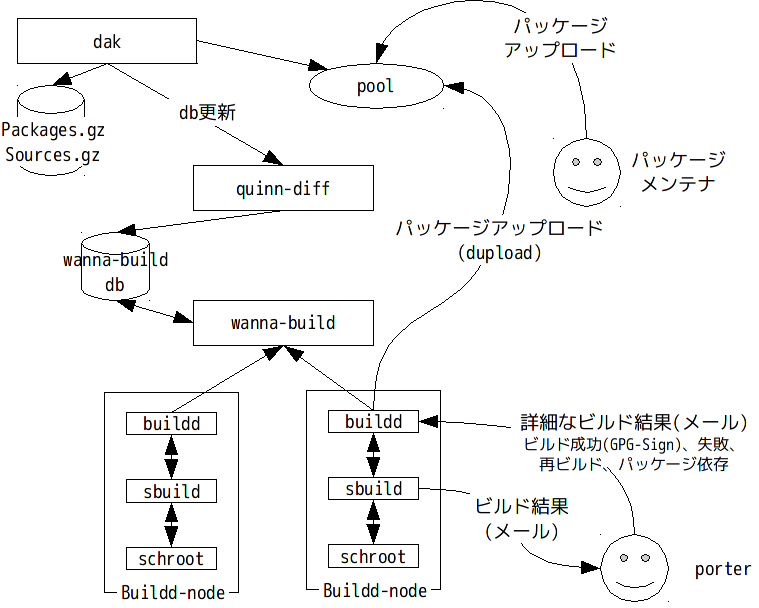
\includegraphics[scale=0.7]{image200911/buildd-image00.png}
 \end{center}
 \caption{コンポーネント連系図}
 \label{fig:buildd-comp}
\end{figure}

\subsection{パッケージの状態遷移}
パッケージは常になにかしらの状態をステータスを持っています。ステータス
は wanna-build で管理する DB で保持されています。
ステータスは以下のものがあり、図\ref{fig:pkg-state}のように変化します。

\begin{itemize}

\item BD-Uninstallable\\
パッケージのビルドに足りないパッケージがある状態。

\item Needs-Build \\
パッケージがビルド可能な状態。
パッケージビルド依存関係が解消されてたり、ビルドの状態から戻された
(given-back) 場合にこの状態になります。

\item Building \\
Builddによってパッケージがビルドされている状態。

\item Uploaded\\
PorterによってパッケージにGPGサインされ、アーカイブにアップロードされた状態。

\item Installed\\
アーカイブにインストールされた状態。

\item Dep-Wait\\
パッケージのビルド依存関係待ちの状態。

\item Failed\\
パッケージがビルドに失敗した状態。

\item Not-For-Us\\
対象のアーキテクチャではビルドできないパッケージの状態。
porterがwanna-build経由でデータベースに登録します。
現在、wanna-build のデータベースとは別にアーキテクチャ依存のリスト
      \footnote{http://buildd.debian.org/git/packages-arch-specific.git}を
作成中です。
\item Failed-Removed\\
Failed 状態のパッケージが一時的に削除されているという状態。

\end{itemize}

\begin{figure}[htbp]
 \begin{center}
   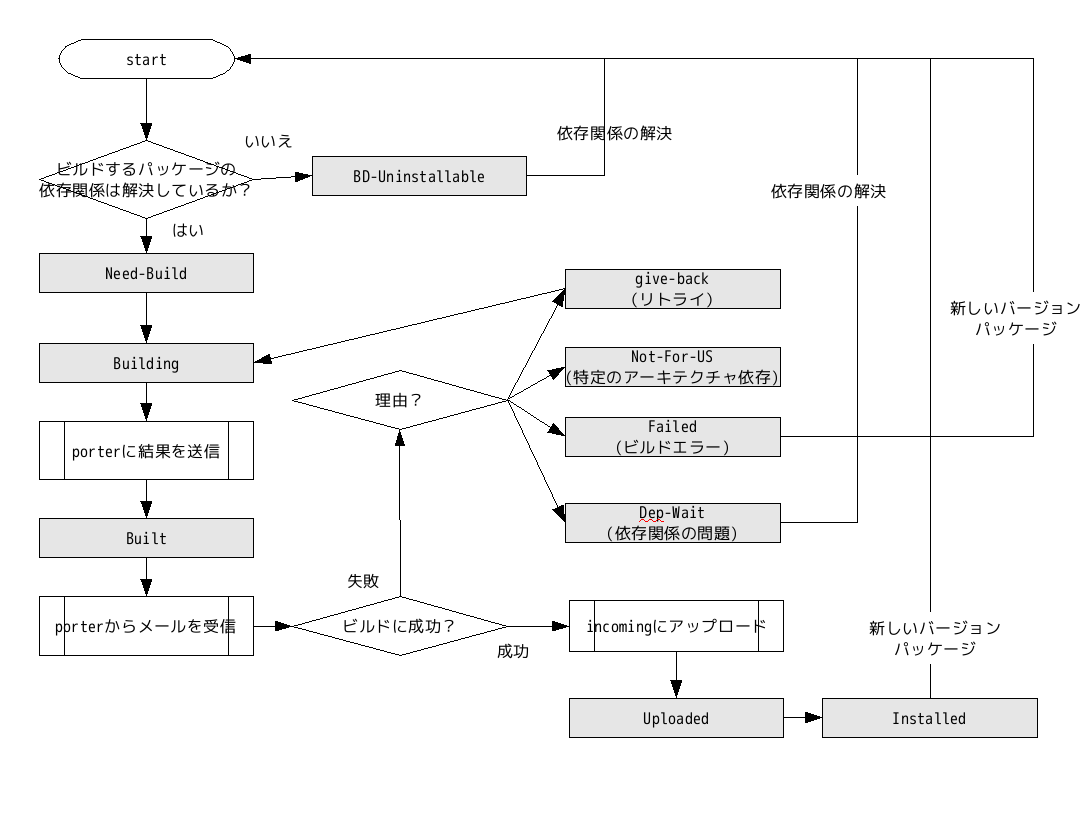
\includegraphics[scale=0.7]{image200911/buildd-status.png}
 \end{center}
 \caption{パッケージステータスの状態遷移}
 \label{fig:pkg-state}
\end{figure}

\subsection{ビルドの優先順位}
パッケージのビルドは基本的に Need-Build のステータスになった順かつパッケー
ジ名ASCII 順でビルドされますが、
それとは別にソースパッケージのプライオリティとソースパッケージのセクション毎に優先順
位が設定されています。現在では、以下の優先順位になっています。

\begin{table}[htbp]
\begin{center}
\begin{tabular}{ccc}

\begin{minipage}{0.3\hsize}
\begin{center}
\begin{tabular}{|c|c|}
\hline
Source Priority & 値 \\ \hline
required & -5 \\ \hline
important & -4 \\ \hline
standard & -3 \\ \hline
optional & -2 \\ \hline
extra & 1 \\ \hline
unknown & -1 \\ \hline
\hline
\end{tabular}
\caption{ソースパッケージプライオリティ毎の優先順位}
\label{tbl:srcpkg-prio}
\end{center}
\end{minipage}

\begin{minipage}{0.3\hsize}
\begin{center}
\begin{tabular}{|c|c|}
\hline
 libs & -200 \\ \hline
 debian-installer & -199 \\ \hline
 base & -198 \\ \hline
 devel & -197 \\ \hline
 shells & -196 \\ \hline
 perl & -195 \\ \hline
 python & -194 \\ \hline
 graphics & -193 \\ \hline
 admin & -192 \\ \hline
 utils & -191 \\ \hline
 x11 & -190 \\ \hline
 editors & -189 \\ \hline
 net & -188 \\ \hline
 mail & -187 \\ \hline
 news & -186 \\ \hline
 tex & -185 \\ \hline
 text & -184 \\ \hline
\hline
\end{tabular}
\caption{ソースパッケージセクション毎の優先順位:その1}
\label{tbl:srcpkg-sec1}
\end{center}
\end{minipage}

\begin{minipage}{0.3\hsize}
\begin{center}
\begin{tabular}{|c|c|}
\hline
 web & -183  \\ \hline
 doc & -182 \\ \hline
 interpreters & -181 \\ \hline
 gnome & -180 \\ \hline
 kde & -179 \\ \hline
 games & -178 \\ \hline
 misc & -177 \\ \hline
 otherosfs & -176 \\ \hline
 oldlibs & -175 \\ \hline
 libdevel & -174 \\ \hline
 sound & -173 \\ \hline
 math & -172 \\ \hline
 science & -171 \\ \hline
 comm & -170 \\ \hline
 electronics & -169 \\ \hline
 hamradio & -168 \\ \hline
 embedded & -166 \\ \hline
 unknown & -165 \\ \hline
\hline
\end{tabular}
\caption{ソースパッケージセクション毎の優先順位:その2}
\label{tbl:srcpkg-sec2}
\end{center}
\end{minipage}

\end{tabular}
\end{center}
\end{table}

\subsection{新しいアーキテクチャをサポートする}

昔は、ポーティングしたい人が quinn-diff から buildd(buildd-node) まで全
て構築する必要がありました。この最大のネックは wanna-build
データベースで、これは最新のものを使う必要があっ
たのですが、データベースにアクセスするにはサーバーのアカウントが必要だっ
たため、
構築が困難でした\footnote{構築は可能だが、タイムラグが発生する。その理由
としてbuilddが参照するリポジトリは最新のリポジトリ情報が反映されるbuildd
専用のため}。しかし、今は新しいアーキテクチャを追加するためのサポー
ト用サービス debian-ports.org が用意されています。このサービスでは、ポー
ティングしたいアーキテクチャ用の
wanna-build 用アカウント と DB, quinn-diff のサービスを提供できるように
なっています。これにより、移植したい人は buildd-node のみを用意し、debian-ports の管理者に登録申請をするだ
けで新しいアーキテクチャをサポートできるようになりました。
現在、\ref{tbl:support-arch}のアーキテクチャが debian-ports.org を使ってポーティ
ングを進めています。

\begin{table}
\begin{center}
\begin{tabular}{|c|c|}
\hline
アーキテクチャ名 & 進捗 \\ \hline
avr32 & 65.52\% \\ \hline
hurd-i386 & 64.46\% \\ \hline
m68k & 53.00\% \\ \hline
sh4 & 85.43\% \\ \hline
\hline
\end{tabular}
\caption{debian-ports.orgでサポート中のアーキテクチャ}
\label{tbl:support-arch}
\end{center}
\end{table}

\subsection{loop-depends の対応方法}

いくつかのパッケージには loop-depends になっているものがあります。
loop-depends とは、ビルド依存がループしているパッケージの状態を言います。
例えば、libpang-perl パッケージ(図\ref{fig:buil-dep-libpango-perl})は
libgtk2-perlパッケージ図\ref{fig:buil-dep-libgtk2-perl}にビルド依存して
います。しかし、libgtk2-perl は libpang-perlパッケージに依存しています。

\begin{figure}[htbp]
\begin{commandline}
Source: libpango-perl
Section: perl
Priority: optional
Build-Depends: debhelper (>= 7.0.50), libcairo-perl (>= 1.000), libextutils-depends-perl (>= 0.300), 
  libextutils-pkgconfig-perl, libglib-perl (>= 1:1.220), perl, xvfb, libpango1.0-dev,
  xauth, xfonts-base, quilt, libgtk2-perl (>= 1:1.220)
                             ^^^^^^^^^^^^^^^^^^^^^^^^^^
\end{commandline}
 \caption{libpango-perlのビルド依存}
 \label{fig:buil-dep-libpango-perl}
\end{figure}

\begin{figure}[htbp]
\begin{commandline}
Source: libgtk2-perl
Section: perl
Priority: optional
Build-Depends: debhelper (>= 7.0.50), quilt (>= 0.46-7), perl, libextutils-depends-perl (>= 0.300), 
 libextutils-pkgconfig-perl (>= 1.03), libgtk2.0-dev (>= 2.6.0), libglib-perl (>= 1:1.220),
 libcairo-perl (>= 1.00), xvfb, xauth, xfonts-base, hicolor-icon-theme,
 libpango-perl (>= 1.220), shared-mime-info
 ^^^^^^^^^^^^^^^^^^^^^^^^^
\end{commandline}
 \caption{libgtk2-perlのビルド依存}
 \label{fig:buil-dep-libgtk2-perl}
\end{figure}

%\begin{figure}[htbp]
% \begin{center}
%   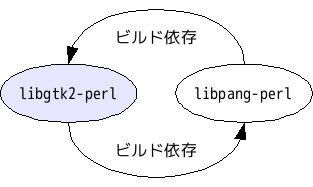
\includegraphics[scale=0.7]{image200911/loop-dep.png}
% \end{center}
% \caption{ループビルド依存関係}
% \label{fig:loop-dep}
%\end{figure}

これではいつになってもビルドできません。これはバグとして扱われるのでは?
と思いますが、libpang-perlをビルドする段階で libgtk2-perlを使ったテス
トを行うため、libgtk2-perlが必要なのです。Debianではソフトウェアのビルド
に実行されるテストは行うことが推奨されているので、このようにビルド依存関係がループしています。
では、どのようにしてビルドすればよいのでしょうか。実は、porterが手を加えてビルドする必要があります。
しかし、手を加えた場合は正式なパッケージとして扱われません。
このようなパッケージに遭遇した場合には、unreleased ディストリビューションにパッケージをアップロードし、
そのパッケージを使って再度ビルドを行うという方法が推奨されています。

以下に例として libpang-perl をビルドする場合の手順を説明します。
\begin{enumerate}

\item builddが動作していない別マシンでの作業
\begin{enumerate}
 \item libpango-perl のソースパッケージをダウンロードします。
 \item debian/control ファイルの Build-depends から libgtk2-perl を削除
       します。
 \item debian/changelog をアップデートします。\\
Debian versionは既存のバージョンに+arch-name などをつける必要があります。
       (実際のDebian packageと区別するため。)
ディストリビューション名は unreleased に変更します。
debian/changelog の変更者も変更する必要があります。
\item debuild -m''Your name $<$your-name@example.org$>$'' などとしてパッケー
      ジをビルドします。 \\
libpango-perlはlibgtk2-perlが見つからない場合には、テストを無視します。:-)
\item ビルドに成功したら、dupload を使ってパッケージアップロードします。
\item dak で処理されれば、unreleased ディストリビューションから libpango-perl が利用できるよ
      うになります。
\end{enumerate}
\item schroot内での作業
\begin{enumerate}
\item schroot環境のapt-lineに unreleased を追加します。
\item schroot内で apt-get update を実行します。
\end{enumerate}
\item libgtk2-perl がビルドできるようになります。
\item libgtk2-perl ができたら、unreleased ディストリビューションから
      libpango-perl を消してもらいます。
\item libpango-perl が 本来のDebian Versionのものでビルドされます。
\end{enumerate}

毎回この方法がうまくいくとは限りません。
例えば、依存するパッケージや提供されるパッケージの機能によっては configure のオ
プションを変更する場合もあります。このあたりはパッケージメンテナか、
debian-wb@l.d.o に直接聞いたほうがよいです。聞かないとわからないというの
は問題なので、README.Debianあたりに書いてもらうように計画中です。

\subsection{まとめ}
auto-builder ネットワークはDebian公式開発者でさえあまり触ることのないシ
ステムです。ブラックボックスなところが以前からあったと思うのですが、
今回の説明で少しはわかる部分が増えたかなと思います。
個人的にはauto と謳っておきながら実は人が介入していたりするのはけっこう
意外でした。auto-builder ネットワークの奥深くに入り込みたい人はぜひ
Debian/SH4のポーティングに参加していただければと思います。

\newpage


%\printindex

\cleartooddpage

\vspace*{15cm}
\hrule
\vspace{2mm}

\includegraphics[width=2cm]{image200502/openlogo-nd.eps}
\noindent \Large \bf Debian 勉強会資料\\ \\
\noindent \normalfont \debmtgyear{}年\debmtgmonth{}月\debmtgdate{}日 \hspace{5mm}  初版第1刷発行\\
\noindent \normalfont 東京エリア Debian 勉強会 (編集・印刷・発行)\\
\hrule


\end{document}
